The virtual-channel allocator is responsible for assigning an available output virtual channel to an input virtual channel. VC allocation is only performed for head flits. When the front flit of an input VC is a head flit, the allocator uses the routing result to identify the requested output port and checks the available output VCs at that port. The availability information is then combined with the candidate VC set to form the final set of allocatable output VCs.

If at least one valid candidate output VC exists, the corresponding input VC sends a request to the separable input-first allocator. The separable allocator then resolves competition among input VCs and output resources using the two-stage arbitration method described previously. When an input VC wins the allocation, the VC allocator generates a grant signal and a one-hot selected output VC signal for that input VC.

After a successful allocation, an update signal is sent to the state unit to mark the selected output VC as occupied. In this way, the VC allocation process can be summarized as three steps: candidate filtering, separable input-first arbitration, and output VC state update. Figure~\ref{fig:vc_allocation_flow} provides an overview of this allocation flow and the relationship among these three stages.

\begin{figure}[htbp]
    \centering
    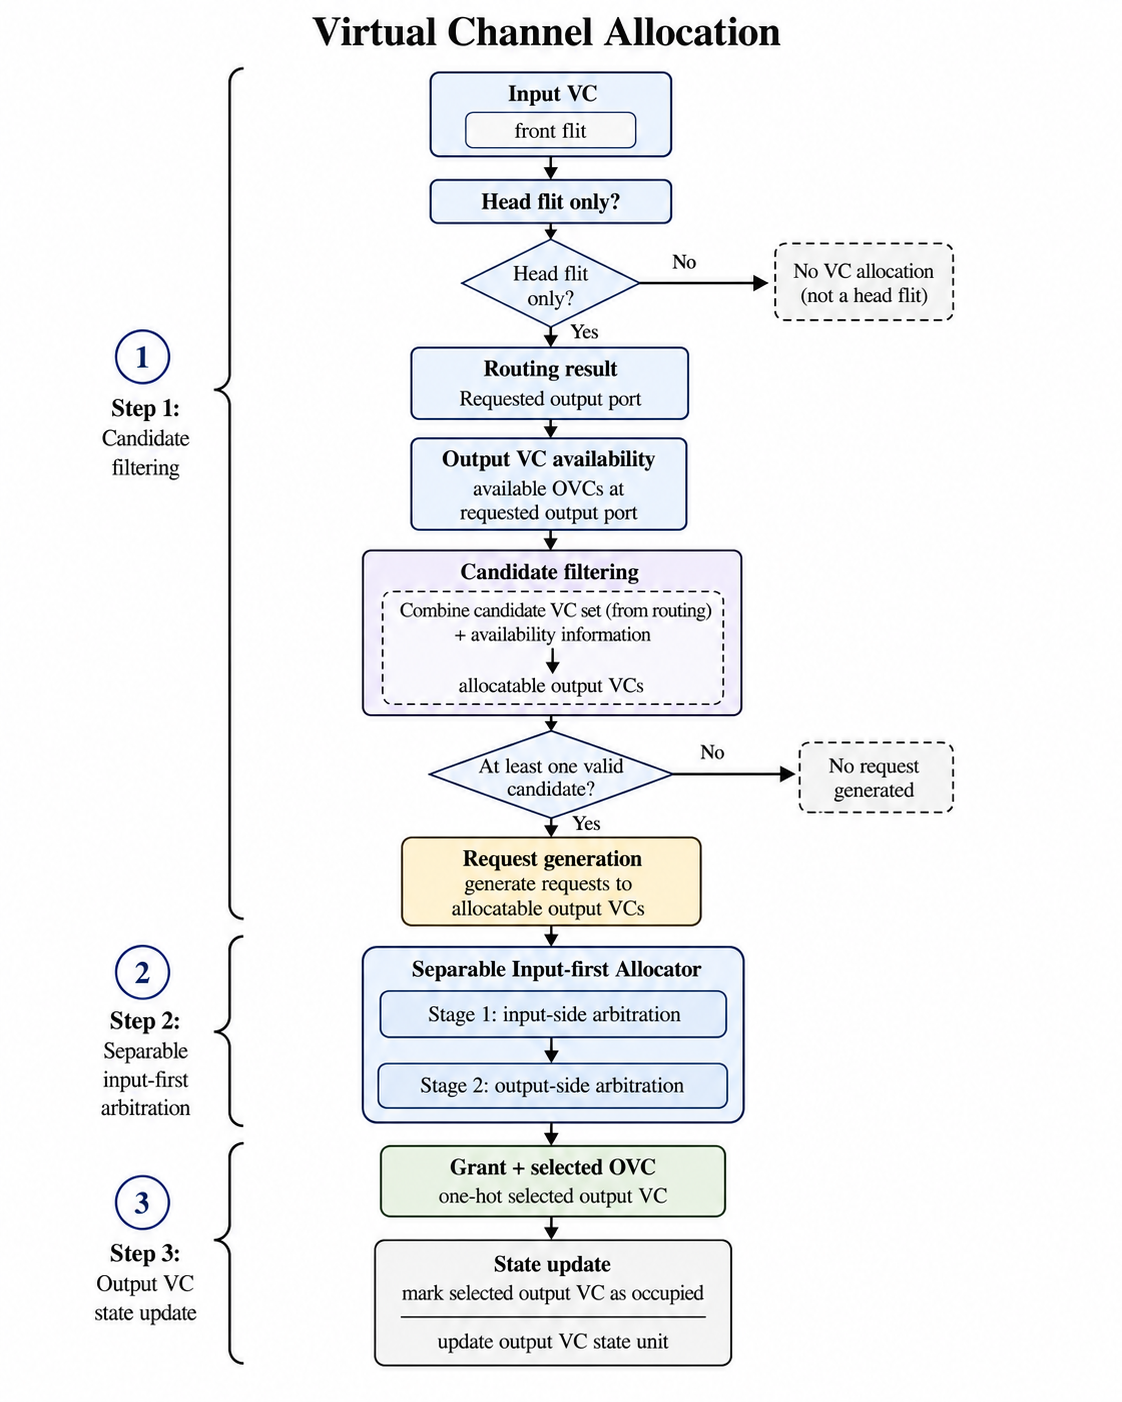
\includegraphics[width=0.8\textwidth]{images/ch3_design_and_implementation/virtual_channel_allocation.png}
    \caption{Virtual-channel allocation flow}
    \label{fig:vc_allocation_flow}
\end{figure}
